\documentclass[../Main.tex]{subfiles}

\begin{document}

\section{Estado del Arte}
Tanto la Agencia Espacial Europea como la NASA han lanzado anteriormente varios concursos públicos de investigación. Entre algunos de estos hay algoritmos de optimización, algoritmos de detección planetaria, prototipos de robots de exploración, desarrollo de aplicaciones móviles, etc.
\newline \par
En relación a los ángulos de incidencia solar, existe una amplia bibliografía sobre la incidencia solar sobre la superficie terrestre. Según el Ngram de Google, este tiene su peak alrededor de 1980, por lo que se considera que estos conceptos tienen una madurez suficiente.
\begin{center}
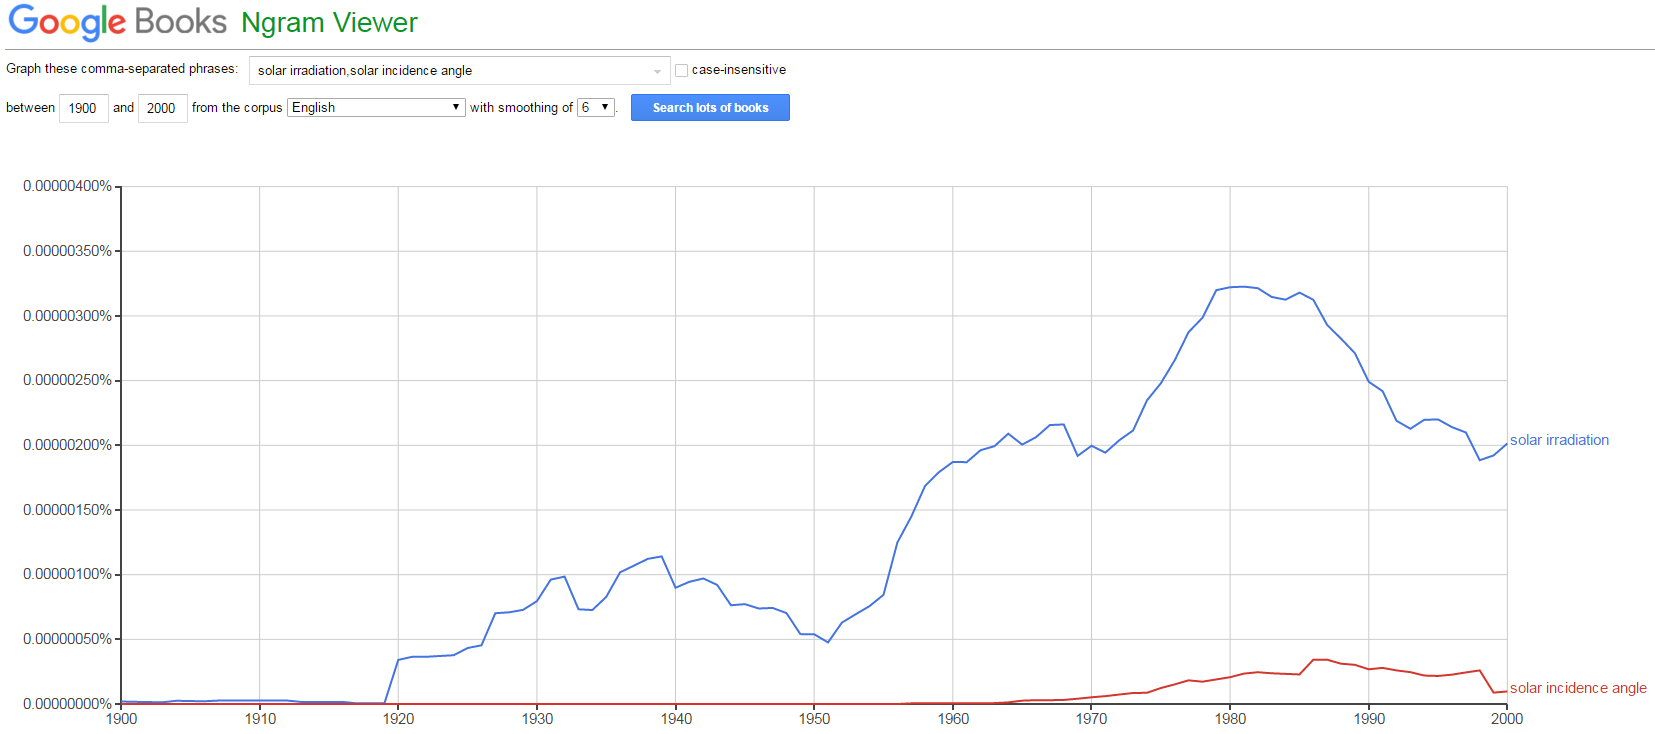
\includegraphics[width=\linewidth, trim={0 0 0 45mm}, clip]{Assets/IncidenciaSolar.PNG}
\\Figura 8. Resultados de búsquedas de incidencia solar e irradiación solar
\end{center}
Para el caso de este proyecto, la incidencia debe ser calculada sobre un satelite, por lo que se prevee se puedan extender los conceptos anteriores.
\newline \par
Con respecto a la información de los sistemas a bordo de la nave, sus comandos y el funcionamiento de los mismos, es poca la información disponible en la página del concurso. Se prevee que el entendimiento de estos sean de poca relevancia, sin embargo se considera que en la medida enque se profundize sobre los datos, se tenga una mejor comprensión sobre los datos anteriores. 
\end{document}